\section{System for elektroniske kalendre}
\subsection{Oversikt over systemet}

Hver ansatt i Firma X skal ha en personlig kalender. Hver gruppe skal ha en gruppe kalender. En gruppe kan bestå av flere personer og også av subgrupper. En person kan være medlem av flere grupper. Alle kalenderne skal være lagret på en kalendertjener. De ansatte skal ha tilgang til kalenderne sine med en kalenderklient. Kalenderklienten kjører på en lokalmaskin som kommuniserer med kalendertjeneren over lokalnettet. Mange kalenderklienter kan være koblet opp mot kalendertjeneren samtidig. Sammen utgjør kalendertjeneren og kalenderklientene systemet som skal implementeres.
Figur \ref{fig:high-level-architecture}  viser et høynivå systemarkitektur over kalendersystemet.

\begin{figure}[H]
    \centering
    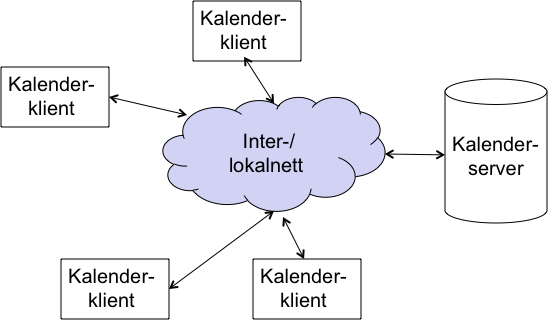
\includegraphics[scale=0.5]{resources/high-level-architecture.png}
    \caption{High level system architecture for calendar system}
    \label{fig:high-level-architecture}
\end{figure}

\subsection{Krav til kalendersystemet}

I tillegg til at de ansatte skal kunne planlegge dagene sine med å legge inn avtaler i kalenderne, er hensikten med kalendersystemet å forenkle innkalling til møter. I dag bruker de ansatte i Firma X mye tid på å koordinere intern-møter i organisasjonen. Tiden går med på å finne tidspunkt som passer for alle møtedeltakere, samt å reservere møterom. Kalendersystemet skal administrere innkalling til møter og reservasjon av møterom.

\begin{enumerate}

\item
Logge på. Ansatte får tilgang til kalendersystemet ved å logge seg på kalenderklienten med brukernavn og passord.

\item
Legge inn avtale. Ansatte skal kunne legge inn avtaler i kalenderene sine. En avtale legges inn på avtaledato med et start- og sluttidspunkt, samt en kort beskrivelse av avtalen ("Bil på verksted") og eventuelt sted for avtalen ("Strandveien Auto").

\item
Slette avtale. Ansatte skal kunne slette en avtale som ligger i en av kalenderene sine.

\item
Endre avtale. Ansatte skal kunne endre på en avtale som ligger i en av kalenderene sine. Alle feltene kan endres.

\item
Kalle inn til møte. En ansatt skal kunne kalle andre ansatte og grupper i Firma X inn til et møte. Den som kaller inn til møte kalles en møteleder. En ansatt skal kunne kalle inn til møte på samme måte som han/hun legger ny avtale inn i en kalender. I tillegg til feltene for en vanlig avtale, inneholder også møteinnkallingen en liste over innkalte møtedeltakere. 

\item
Motta møteinnkalling. Når en ansatt mottar innkalling til et møte, kan han/hun svare 'Godta' eller 'Forkast'. Ved å svare 'Godta', legges møteinnkallingen inn som en avtale i den innkalte ansattes kalender. Om den ansatte svarer 'Avslag', sendes svar tilbake til møtelederen om at innkallingen ikke er godtatt. Møteleder kan da velge å finne et nytt tidspunkt, avlyse møtet (se under) eller fjerne deltakeren fra innkallingslista.

\item
Endre møteinnkalling. Møteleder kan endre tidspunkt på en møteinnkalling. Det sendes da beskjed ut til alle møtedeltakerne, som kan svare 'Godta' eller 'Forkast'. Ved å svare 'Godta', endres avtalen i den innkalte ansattes kalender. Ved å svare 'Forkast' sendes beskjed ut til alle innkalte møtedeltakere. Møteleder kan da velge å finne et nytt tidspunkt eller å avlyse møtet (se under).

\item
Avlyse møte. Møteleder kan avlyse et møte. Det sendes da beskjed til alle møtedeltakerne, og systemet sletter møtet i deltakernes personlige kalender.

\item
Melde avbud for møte. En ansatt kan melde avbud på en møteinnkalling ved å slette avtalen i sin personlige kalender. Når en ansatt melder avbud, sendes melding til alle de andre møtedeltakerne. Møteleder kan da velge om møtet skal avlyses eller om han/hun skal endre tidspunkt på møtet.

\item
Reservere møterom. I stedet for å skrive inn sted for en avtale eller et møte, skal brukeren kunne reservere møterom. Kalendertjeneren skal lage en liste med tilgjengelige møterom (tilgjengelig betyr ikke reserverte) i tidsperioden for avtalen/møtet. Brukeren kan da velge møterom fra denne listen. Om en avtale med reservert møterom slettes, skal reservasjonen slettes på kalendertjeneren. Det samme gjelder for møter som avlyses.

\item
Visning. Kalenderklienten skal vise en ukekalender der alle avtaler og møter i den ansattes personlige kalender vises. Det skal være enkelt å bla mellom ukene.

\item
Spore møteinnkallinger. Kalenderklienten skal indikere i ukekalenderen om a) en møteinnkalling venter på svar fra en eller flere deltakere, b) en eller flere møtedeltakere har avslått møteinnkalling, eller c) om alle innkalte har godtatt møteinnkallingen.

\item
Vis flere kalendre. Det skal være mulig å vise andre ansattes avtaler sammen med sine egne i kalenderklienten.

\item
Alarm. Det skal være mulig for hver ansatt å konfigurere enhver avtale slik at avtalen genererer en alarm en gitt tid før møtet. 

\end{enumerate}

\subsection{Scenarioer}

Scenarioene er ikke en del av kravspesifikasjonen, men skisserer noen typiske bruksscenarier for kalendersystemet.

\begin{enumerate}

\item
En ansatt har invitert tre forretningsforbindelser til samtaler i Firma X sine lokaler. Den ansatte legger inn dette som en avtale i kalenderen sin, og får kalendersystemet til å booke et ledig møterom som er passe stort for fire deltakere.

\item
Jens kaller Beate, Morten og Finn til møte. Kalendersystemet  førstkommende fredag klokka 12 til 14. Kalendertjeneren sender melding til de tre Jens har kalt inn til møte. Morten er logget på systemet med en klient, og mottar øyeblikkelig melding om møteinnkallingen. Beate og Finn mottar meldingen neste gang de logger på.

\item
Beate avslår møteinnkallingen fordi hun har en annen avtale på det tidspunktet. Morten og Finn godtar innkallingen. Først forsøker Jens seg med å endre tidspunktet på møtet. Kalendertjeneren sender ny melding ut til møtedeltakerne. Denne gangen godtar både Beate og Finn møteinnkallingen, men Morten avslår. Jens velger å slette Morten fra møteinnkallingen. 

\item
Etter at Beate og Finn har godtatt møteinnkallingen blir Jens syk. Han sletter møtet fra kalenderen sin. Kalendertjeneren sender da melding til de to andre deltakerne om at møtet er avlyst. Beate og Finn mottar begge denne meldingen neste gang de logger seg på kalendersystemet.

\end{enumerate}
